\documentclass[a4paper,12pt,oneside]{report}
\usepackage{titlesec}
\usepackage[svgnames]{xcolor}
%\usepackage[usenames,dvipsnames]{color}
\usepackage[top=0cm,bottom=0cm,left=0cm,right=0cm]{geometry}
%\usepackage{fullpage}
\usepackage[utf8]{inputenc}
\usepackage[T1]{fontenc}
\usepackage{graphicx}
\usepackage{wallpaper}
\usepackage{wrapfig}
\usepackage{hyperref}
\usepackage[francais]{babel}
%\usepackage{color}
\usepackage{layout}
\usepackage{circuitikz}
\usepackage[squaren, Gray]{SIunits}
\usepackage{sistyle}
\usepackage[autolanguage]{numprint}

%Algo package
\usepackage[ruled,vlined]{algorithm2e}
\usepackage{algpseudocode}

\usepackage{array}
\usepackage{calc}

\hypersetup{pdfborder={0 0 0}}

\titleformat{\part}
{\centering\fontfamily{pag}\fontsize{30}{30}\selectfont}
{\fontfamily{pag}\fontsize{30}{30}\selectfont Partie \ \thepart \ - }
{0pt}
{}{}

%Modifie le format des chapitres
\titleformat{\chapter}
{\it \color{DodgerBlue} \fontfamily{pag}\fontsize{20.74}{20}\selectfont}
{\it \fontfamily{pag}\fontsize{20.74}{20}\selectfont Chapitre \ \thechapter \ - }
{0pt}
{}{}
\titlespacing{\chapter}{0pt}{0.5cm}{0.5cm}[0pt]

%Modifie le format des sections
\titleformat{\section}
{\color{LimeGreen}\fontfamily{pag}\fontsize{15}{15}\selectfont}
{\fontfamily{pag}\fontsize{15}{15}\selectfont \thesection }
{5pt}
{}{}
\titlespacing{\section}{1cm}{0.5cm}{0.25cm}[0cm]

%Modifie le format des sous-secions
\titleformat{\subsection}
{\color{DarkOrange}\fontfamily{pag}\fontsize{12}{12}\selectfont}
{\fontfamily{pag}\fontsize{12}{12}\selectfont \thesubsection}
{5pt}
{}{}
\titlespacing*{\subsection}{2cm}{0.1cm}{0.1cm}[0cm]

%Modifie l'espace avant les paragraphes
\setlength{\parindent}{0pt}
\makeatletter

\newcommand{\bigO}{$\mathcal{O}$}

% Commande créeant une page de titre
%	#1=Titre
%	#2=Sous-titre
%	#3=Auteur
%	#4=image
%	#5=couleur de fond
%	#6=couleur cadre titre,sous-titre,auteur
\newcommand{\titre}[6]
{
	\begin{document}
	\begin{titlepage}
		\pagecolor{#5} % met la couleur de la page
		\vspace*{0.6cm}\fontfamily{pag}\fontsize{20}{20}\selectfont{\begin{center}2015-2016\end{center}}\vspace*{0.3cm}	% insère l'année en haut de la page
		\vspace*{-0.1cm}
		\includegraphics[width=\paperwidth]{#4} % insère l'image
		\colorbox{#6}{	%boîte de couleur avec le titre, sous-titre et l'auteur
			\hspace*{1.2cm}
			\begin{minipage}{\textwidth-1.8cm}{
				\vspace*{1cm}
				\begin{flushleft}\bfseries
					\fontfamily{pag}\fontsize{35}{35}\selectfont{#1}	%Titre
					\vspace*{0.5cm}
				\end{flushleft}
				\begin{flushleft}
					\fontfamily{pag}\fontsize{30}{30}\selectfont{#2}	%Sous-Titre
				\end{flushleft}
				\vspace*{1cm}
				\begin{flushright}
					\fontfamily{pag}\fontsize{20}{20}\selectfont{#3}	%Auteur
				\end{flushright}}
			\vspace*{1cm}
			\end{minipage}}
			\begin{center}
				\vfill % repli le reste de la page
				\fontfamily{pag}\fontsize{20}{20}\selectfont{\today} 	%Date
			\end{center}
	\end{titlepage} % fin de la page de titre
	\color{black} % met la couleur du reste du texte à noir
	\pagecolor{white}	% met la couleur des pages suivante à blanc
	\newgeometry{top=1.5cm,bottom=1.5cm,left=1cm,right=1cm}	% modification des marges
	\tableofcontents	%tables des matières
}
\titre{ELEC-1370 Circuits \& Mesures}{Synthèse}{Damien Deprez}
\chapter{Concepts de base}
Le courant est défini comme étant le flux de charge passant à travers un matériau. Il se note $I$.
$$i(t)=\frac{dq(t)}{dt}$$
où $q$ représente la charge.

\chapter{Circuit Résistif}
\section{Loi d'Ohm}
La loi d'Ohm dit : \emph{La tension au borne d'une résistance est directement proportionnel au courant qui la traverse}. Sous forme mathématique cela donne.
\begin{equation}
v(t)=Ri(t) [\unit{}{\ohm}]
\end{equation}
La puissance dissipée dans un résistance est donné par $p(t)=v(t)i(t)$.

On défini aussi la conductance noté $G[ \unit{}{\siemens}]$. C'est l'inverse de la résistance $G=\dfrac{1}{R}$.
\section{Loi de Kirchhoff}
\subsection{Loi des nœuds (KCL)}
La loi des nœuds dit \emph{en chaque nœud, la somme des courant doit être nulle}. De manière mathématique
\begin{equation}
\sum_{j=1}^{N}{i_j(t)}=0  
\end{equation}
\begin{figure} [!h]
\centering
\begin{circuitikz} [american currents, american voltages]
\draw 
%symbole

(0,3) to [I, i=$i_1$] (0,6)
(0,0) to [R, l=$R_4$, i_<=$i_6$, -*] (0,3)
(0,3) to [R, l=$R_3$, i_<=$i_4$, *-*] (3,3)
(3,3) to [R, l=$R_1$, i<=$i_2$, -*] (3,6)
(3,0) to [V, v=$v_2$, i<^=$i_7$, *-*] (3,3)
(6,3) to [V, v=$v_1$, i>^=$i_5$] (3,3)
(6,6) to [R, l=$R_2$, i>^=$i_3$] (6,3)
(6,0) to [R, l=$R_5$, i>^=$i_8$, -*] (6,3)

%couleur
(0,0) to [R, color=blue] (0,3)
(0,3) to [R, color=blue] (3,3)
(3,3) to [R, color=blue]  (3,6)
(6,6) to [R, color=blue] (6,3)
(6,0) to [R, color=blue] (6,3)
(3,0) to [V, color=red] (3,3)
(6,3) to [V, color=red] (3,3)
(0,3) to [I, color=red] (0,6)

%fil
(0,0) -| (3,0) -| (6,0) 
(0,6) -| (3,6) -| (6,6)

%noeud
(3,6) node [above] {1}
(0,3) node [left] {2}
(3,3) node [above right] {3}
(6,3) node [right] {4}
(3,0) node [below] {5}
;
\end{circuitikz}
\caption{Exemple 1 : Application de KCL}
\end{figure}

En appliquant la loi des nœuds, on obtient comme système d'équation
$$
\left\{
\begin{array} {r c l}
i_1 - i_2 -i_3 & = & 0\\
i_4-i_1-i_6&=&0\\
i_2 - i_4 + i_5 - i_7 &=& 0\\
i_3+i_8-i_5&=&0\\
i_6-i_7-i_8&=&0
\end{array}
\right.
$$
\subsection{Loi des mailles (KVL)}

La loi des mailles dit \emph{La somme des tensions dans une boucle fermée doit être nulle}. De manière mathématique
\begin{equation}
\sum_{j=1}^{N}{v_j(t)}=0  
\end{equation}

\section{Montage de plusieurs résistances}
\subsection{montage série}
Dans un montage série, le courant passant à travers chaque élément est le même. On peut remplacer ce montage par une seule résistance dont la valeur vaut la somme des résistances mise en série
\begin{equation}
R_p=\sum_{j=1}^{N}{R_j}
\end{equation}

\subsection{montage parallèle}
Dans un montage parallèle, la tension est la même aux bornes de chaque élément. On peut remplacer ce montage par une seule résistance $R_p$ dont la valeur vaut l'inverse de la somme des inverses des résistances montées en parallèle.
\begin{equation}
R_p=\frac{1}{\sum_{j=1}^{N}{\frac{1}{R_j}}}
\end{equation}

\subsection{montage triangle-étoile}

La figure \ref{figure:triangle-etoile} montre le montage en triangle sur la gauche et le montage ne étoile sur la droite. 
\begin{figure} [!h]
\centering
%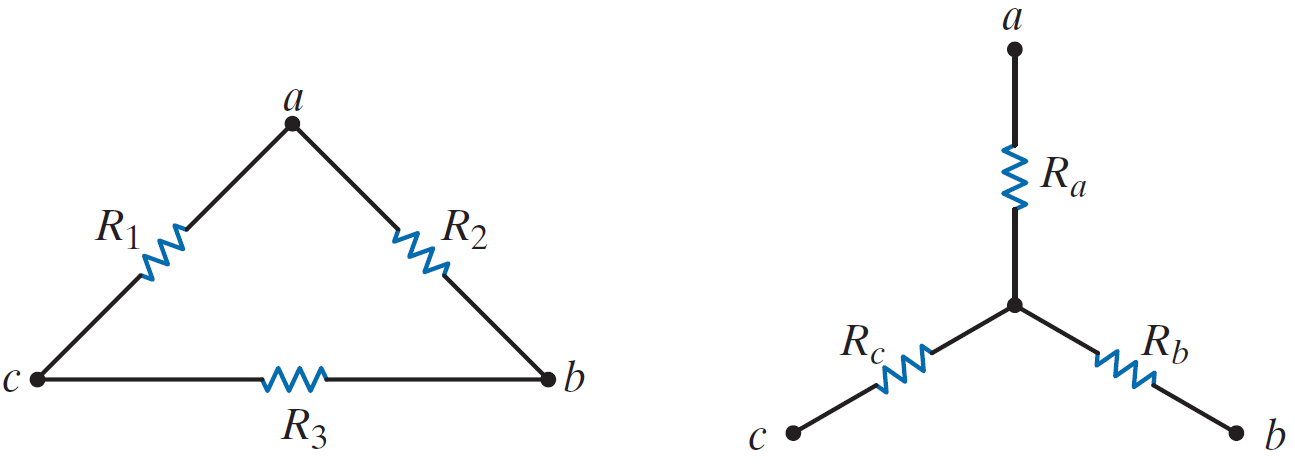
\includegraphics[width=0.8\textwidth]{img/triangleetoile}
\begin{circuitikz} [american currents, american voltages]
\ctikzset {label/align = straight}
\draw

%symbole
(0,0) to [R, l=$R_1$,*-*] (3,3)
(3,3) to [R, l=$R_2$,*-*] (6,0)
(6,0) to [R, l=$R_3$, *-*] (0,0)

%couleur
(0,0) to [R, color=blue] (3,3)
(3,3) to [R, color=blue] (6,0)
(6,0) to [R, color=blue] (0,0)

%noeud
(0,0) node [left] {$c$}
(3,3) node [above] {$a$}
(6,0) node [right] {$b$}
;
\end{circuitikz} \hspace*{2cm}
\begin{circuitikz}[american currents, american voltages]
\ctikzset {label/align = straight}
\draw

%symbole
(0,0) to [R, l=$R_c$,*-*] (3,2)
(3,4) to [R, l=$R_a$,*-*] (3,2)
(3,2) to [R, l=$R_b$, *-*] (6,0)

%couleur
(0,0) to [R, color=blue] (3,2)
(3,4) to [R, color=blue] (3,2)
(6,0) to [R, color=blue] (3,2)

%noeud
(0,0) node [left] {$c$}
(3,4) node [above] {$a$}
(6,0) node [right] {$b$}
;

\end{circuitikz}
\caption{\label{figure:triangle-etoile}Montage en triangle à gauche et montage en étoile à droite}
\end{figure}
Pour passer du montage triangle au montage en étoile, on utilise les formules suivantes
$$R_a=\dfrac{R_1R_2}{R_1+R_2+R_3}$$
$$R_b=\dfrac{R_2R_3}{R_1+R_2+R_3} $$
$$R_c=\dfrac{R_1R_3}{R_1+R_2+R_3} $$

Pour passer du montage en étoile au montage en triangle, on utilise les formules suivantes
$$R_1=\frac{R_aR_b+R_bR_c+R_aR_c}{R_b}$$
$$R_2=\frac{R_aR_b+R_bR_c+R_aR_c}{R_c}$$
$$R_3=\frac{R_aR_b+R_bR_c+R_aR_c}{R_a}$$
\newpage
\section{Dipôle équivalent}
\subsection{Équivalent de Thévenin}
Le circuit équivalent de Thévenin est montré sur la figure \ref{fig:thevenin} où la tension de Thévenin vaut la tension en circuit ouvert ($v_{oc}$).

\begin{figure} [!h]
\centering
\begin{circuitikz} [american voltages, american currents]
\draw

%symbole
(0,0) to [V, l=$v_{oc}$] (0,2)
(0,2) to [R, l=$R_{Th}$, i>^=$i$, -o] (3,2)

%couleur
(0,0) to [V, color=red] (0,2)
(0,2) to [R, color=blue] (3,2)

%fil
(0,0) to [short, -o] (3,0)

%noeud
(3,0) node [above] {B}
(3,2) node [below] {A}
;
\end{circuitikz}

\caption{\label{fig:thevenin}Circuit équivalent de Thévenin}
\end{figure}

\subsection{Circuit équivalent de Norton}
Le circuit équivalent de Norton est montré sur la figure \ref{fig:norton} où le courant de Norton vaut le courant en court-circuit ($i_{sc}$).
\begin{figure} [!h]
\centering
\begin{circuitikz} [american voltages, american currents]
\draw
%symbole
(0,0) to [I, i=$i_{sc}$] (0,2)
(2,0) to [R, l=$R_{No}$] (2,2)

%couleur
(0,0) to [I, color=red] (0,2)
(2,0) to [R, color=blue] (2,2)

%fil
(2,2) to [short, -o, i>=$i$] (3,2)
(2,0) to [short, -o] (3,0)
(0,0) -| (2,0)
(0,2) -| (2,2)

%noeud
(3,0) node [above] {B}
(3,2) node [below] {A}
;
\end{circuitikz}
\caption{\label{fig:norton}Circuit équivalent de Norton}
\end{figure}
\subsection{Relation entre les équivalents de Norton et Thévenin}
La relation qui existe entre les équivalents de Norton et de Thévenin est la suivante
\begin{equation}
v_{oc}=i_{sc}R_{Th}
\end{equation}

\chapter{Quadripôle à deux accès}
Tout comme pour les dipôles équivalents pour les circuits à deux bornes, il existes des quadripôles équivalents pour les circuits à quatre bornes. Les conventions des accès à un quadripôles sont repris sur la figure \ref{fig:in-out_quadripole}. Un quadripôle ne doit pas contenir de source de tension ou de courant indépendante. 
\begin{figure} [!h]
\centering
\input{circuit/schema_quadripole.cir}
\caption{\label{fig:in-out_quadripole}Entrée et sortie d'un quadripôle}
\end{figure}
\section{Représentations}
Il existe plusieurs manière de représenter un quadripôle sous forme de réseaux de Kirchhoff. Dans le cadre du cours, quatre représentation on été vue. Il s'agit des représentations
\begin{itemize}
\item Y : Trans-admittances
\item Z : Trans-impédances
\item G : Gain en tension
\item H : Gain en courant
\end{itemize}
\subsection{Représentation sous-circuit}
\begin{figure} [!h]
\centering
\input{circuit/representation_quadripole.cir}
\caption{\label{fig:representation_quadripole}Représentation Y,Z, G et H sous forme de réseaux de Kirchhoff}
\end{figure}
\subsection{Représentation matricielle}
\paragraph*{}
\begin{minipage}[c]{9cm}
\begin{center}Représentation Y\end{center}
\begin{itemize}
\item $y_i$: admittance d'entrée
\item $y_r$: trans-admittance inverse (reverse)
\item $y_f$: trans-admittance directe (forward)
\item $y_o$: admittance de sortie
\end{itemize}
\vspace{0.5cm}
\[
\begin{bmatrix}
i_i\\
i_o
\end{bmatrix}
=
\begin{bmatrix}
y_i & y_r\\
y_f & y_o
\end{bmatrix}
\begin{bmatrix}
v_i\\
v_o
\end{bmatrix}
\]
\end{minipage}
\begin{minipage}[c]{9cm}
\begin{center}Représentation G\end{center}
\begin{itemize}
\item $g_i$: admittance d'entrée
\item $g_r$: gain en courant
\item $g_f$: gain en tension
\item $g_o$: impédance de sortie
\end{itemize}
\vspace{0.5cm}
\[
\begin{bmatrix}
i_i\\
v_o
\end{bmatrix}
=
\begin{bmatrix}
g_i & g_r\\
g_f & g_o
\end{bmatrix}
\begin{bmatrix}
v_i\\
i_o
\end{bmatrix}
\]
\end{minipage}
\paragraph*{}
\begin{minipage}[c]{9cm}
\begin{center}Représentation Z\end{center}
\begin{itemize}
\item $z_i$: impédance d'entrée
\item $z_r$: trans-impédance inverse (reverse)
\item $z_f$: trans-impédance directe (forward)
\item $z_o$: impédance de sortie
\end{itemize}
\vspace{0.5cm}
\[
\begin{bmatrix}
v_i\\
v_o
\end{bmatrix}
=
\begin{bmatrix}
z_i & z_r\\
z_f & z_o
\end{bmatrix}
\begin{bmatrix}
i_i\\
i_o
\end{bmatrix}
\]
\end{minipage}
\begin{minipage}[c]{9cm}
\begin{center}Représentation H\end{center}
\begin{itemize}
\item $h_i$: impédance d'entrée
\item $h_r$: gain en tension
\item $h_f$: gain en courant
\item $h_o$: admittance de sortie
\end{itemize}
\vspace{0.5cm}
\[
\begin{bmatrix}
v_i\\
i_o
\end{bmatrix}
=
\begin{bmatrix}
h_i & h_r\\
h_f & h_o
\end{bmatrix}
\begin{bmatrix}
i_i\\
v_o
\end{bmatrix}
\]
\end{minipage}
\chapter{Circuit en régime sinusoïdale}
\section{Régime sinusoïdale}
Lorsqu'un circuit est alimenté par une source sinusoïdale, la réponse du circuit est donné par l'équation différentielle suivante
\begin{equation}
\sum_{i=n}^{1}{a_i\dfrac{d^i}{dt^i}f(t)}+a_0f(t)=b_s\cos (\omega t)
\end{equation}
où $b_s$ est la source de tension ou de courant indépendante et $f$ la tension d'un nœud ou le courant d'une branche du circuit.
Pour un circuit \emph{stable}, la solution est de la forme 
\begin{equation}
f(t)=kb_s\left[T(s)+\cos(\omega t + \phi) \right]
\end{equation}
Lorsque $t$ est grand ($t\rightarrow\infty$), la solution est de la forme 
\begin{equation}
f(t)=kb_s\cos(\omega t + \phi)
\end{equation}
Cette solution est dite la solution en régime.
\section{Représentation avec des phaseurs}
En régime sinusoïdale, on peu aussi représenter une tension ou un courant sous forme complexe. Cela se fait à l'aide des phaseurs.
\begin{equation}
v(t)=V_M e^{j\phi}=V_M\angle\phi \text{ et  } i(t)=I_Me^{j\phi}=I_M\angle\phi
\end{equation}
\subsection{Équation constitutives des différents éléments en terme de phaseurs}
\begin{tabular}{l | c | c | c | c | c }
\textbf{Élément} & \textit{Source de tension} & \textit{Source de courant} & \textit{Résistance} & \textit{Inductance} & \textit{Condensateur}\\
\hline
\textbf{Paramètre} & $V_0$ & $I_0$ & $R$ & $L$ & $C$\\
Impédance ($Z$) & & & $Z=R$ & $Z=j\omega L$ &$Z=\dfrac{1}{J\omega C}$\\
Admittance ($Y$) & & & $Y=\dfrac{1}{R}$ & $Y=\dfrac{1}{j\omega L}$ & $Y=j\omega C$ \\
\hline
\multirow{2}*{\textbf{Équation constitutive}} & \multirow{2}*{$V=V_0e^{j/phi}$} & \multirow{2}*{$I=I_0e^{j/phi}$} & \multicolumn{3}{c }{$ V = Z I$}\\
& & & \multicolumn{3}{c }{$I = Y V$}\\
\hline
\end{tabular}
\subsubsection{Impédance \& Admittance}
\paragraph{Impédance d'un dipôle}
L'impédance d'un dipôle se note $\textbf{Z}$. Elle est définie comme le rapport du phaseur de tension sur le phaseur de courant.
\begin{equation}
\textbf{Z}[\Omega]=\frac{\textbf{V}}{\textbf{I}}=\frac{V}{I}e^{j(\psi_V-\psi_I)}=\frac{V}{I}e^{j\phi}
\end{equation}
avec comme convention que $\phi$ est la phase de la tension par rapport à la phase du courant.
L'impédance peut se noter sous forme polaire ou cartésienne
\[
\textbf{Z}=|\textbf{Z}|e^{j\arg(\textbf{Z})}=Ze^{j\phi}=R+jX
\]
avec $R$ la résistance et $X$ la réactance.
\paragraph{Admittance d'un dipôle}
L'admittance notée $\textbf{Y}$ est définie comme le rapport du phaseur de courant sur le phaseur de tension.
\begin{equation}
\textbf{Y}[\text{S}]=\frac{\textbf{I}}{\textbf{V}}=\frac{I}{V}e^{-j\phi}
\end{equation}
L'admittance peut se noter sous forme polaire ou cartésienne
\[
\textbf{Y}=|\textbf{Y}|e^{j\arg(\textbf{Y})}=Ye^{-j\phi}=G+jB
\]
avec $G$ la conductance et $B$ la susceptance.

\paragraph{Remarque} Dans le domaine phasoriel, les lois de Kirchhoff, la loi d'Ohm, les dipôles équivalents restent valable.

\chapter{Comportement des circuits dans le domaine fréquentiel}
\section{Diagramme de Bode}
Le diagramme de Bode est utilisé pour visualiser et communiquer de l'information sur la 
réponse en fréquence d'un système. Il est constitué de deux diagrammes :
\begin{itemize}
\item le diagramme en amplitude
\item le diagramme des phases
\end{itemize}
Sur le diagramme en amplitude, on mesure l'amplitude en \unit{}{\deci\bel}. Les \unit{}{\deci\bel} sont défini à partir des gains de puissance.
\begin{equation}
\unit{}{\deci\bel}\left(\dfrac{p_2}{p_1}\right) =10\log_{10}\left(\dfrac{p_2}{p_1}\right)
\end{equation}
On peut aussi définir les \unit{}{\deci\bel} à partir des gains en tension ou en courant.
\begin{equation}
\unit{}{\deci\bel}\left(\dfrac{v_2}{v_1}\right) =10\log_{10}\left(\dfrac{v_2^2}{v_1^2}\right)=20log_{10}\left(\dfrac{v_2}{v_1}\right)
\end{equation}
Sur le diagramme en amplitude, on affiche 
\begin{equation}
\unit{}{\deci\bel}\left(|H|\right)
\end{equation}
où $|H|$ est le module de $H$.

L'équation générale de $H(\omega)$ est : 
\begin{equation}
H(j\omega)=A(j\omega)^{\pm N}\dfrac{\left(1+\dfrac{j\omega}{\omega_1}\right)\left(1+2j\xi_a\dfrac{\omega}{\omega_a}-\left[\dfrac{\omega}{\omega_a}\right]^2\right)}{\left(1+\dfrac{j\omega}{\omega_2}\right)\left(1+2j\xi_b\dfrac{\omega}{\omega_b}-\left[\dfrac{\omega}{\omega_b}\right]^2\right)}
\end{equation}

Sur le diagramme de phase, on affiche
\begin{equation}
\arg (H) \unit{}{[\deg]}
\end{equation}

Lorsque $$H=1+2j\xi  \dfrac{\omega}{\omega_0}-\left(\dfrac{\omega}{\omega_0}\right)^2=\left(1+j\dfrac{\omega}{\omega_1}\right).\left(1+j\dfrac{\omega}{\omega_2}\right)$$ on a comme solution $\omega_{1,2}=\xi\omega_0 \pm \omega_0\sqrt{\xi^2-1}$
$$  $$ ce circuit est dit résonnant si $\xi<1$. Dans ces circuits, on appelle $Q$ le facteur de qualité qui vaut $\frac{1}{2\xi}$. Dès lors, on peut déterminer la bande passante : $\frac{\omega_0}{Q}=2\xi\omega_0$
%\begin{figure}[!h]
%\centering
%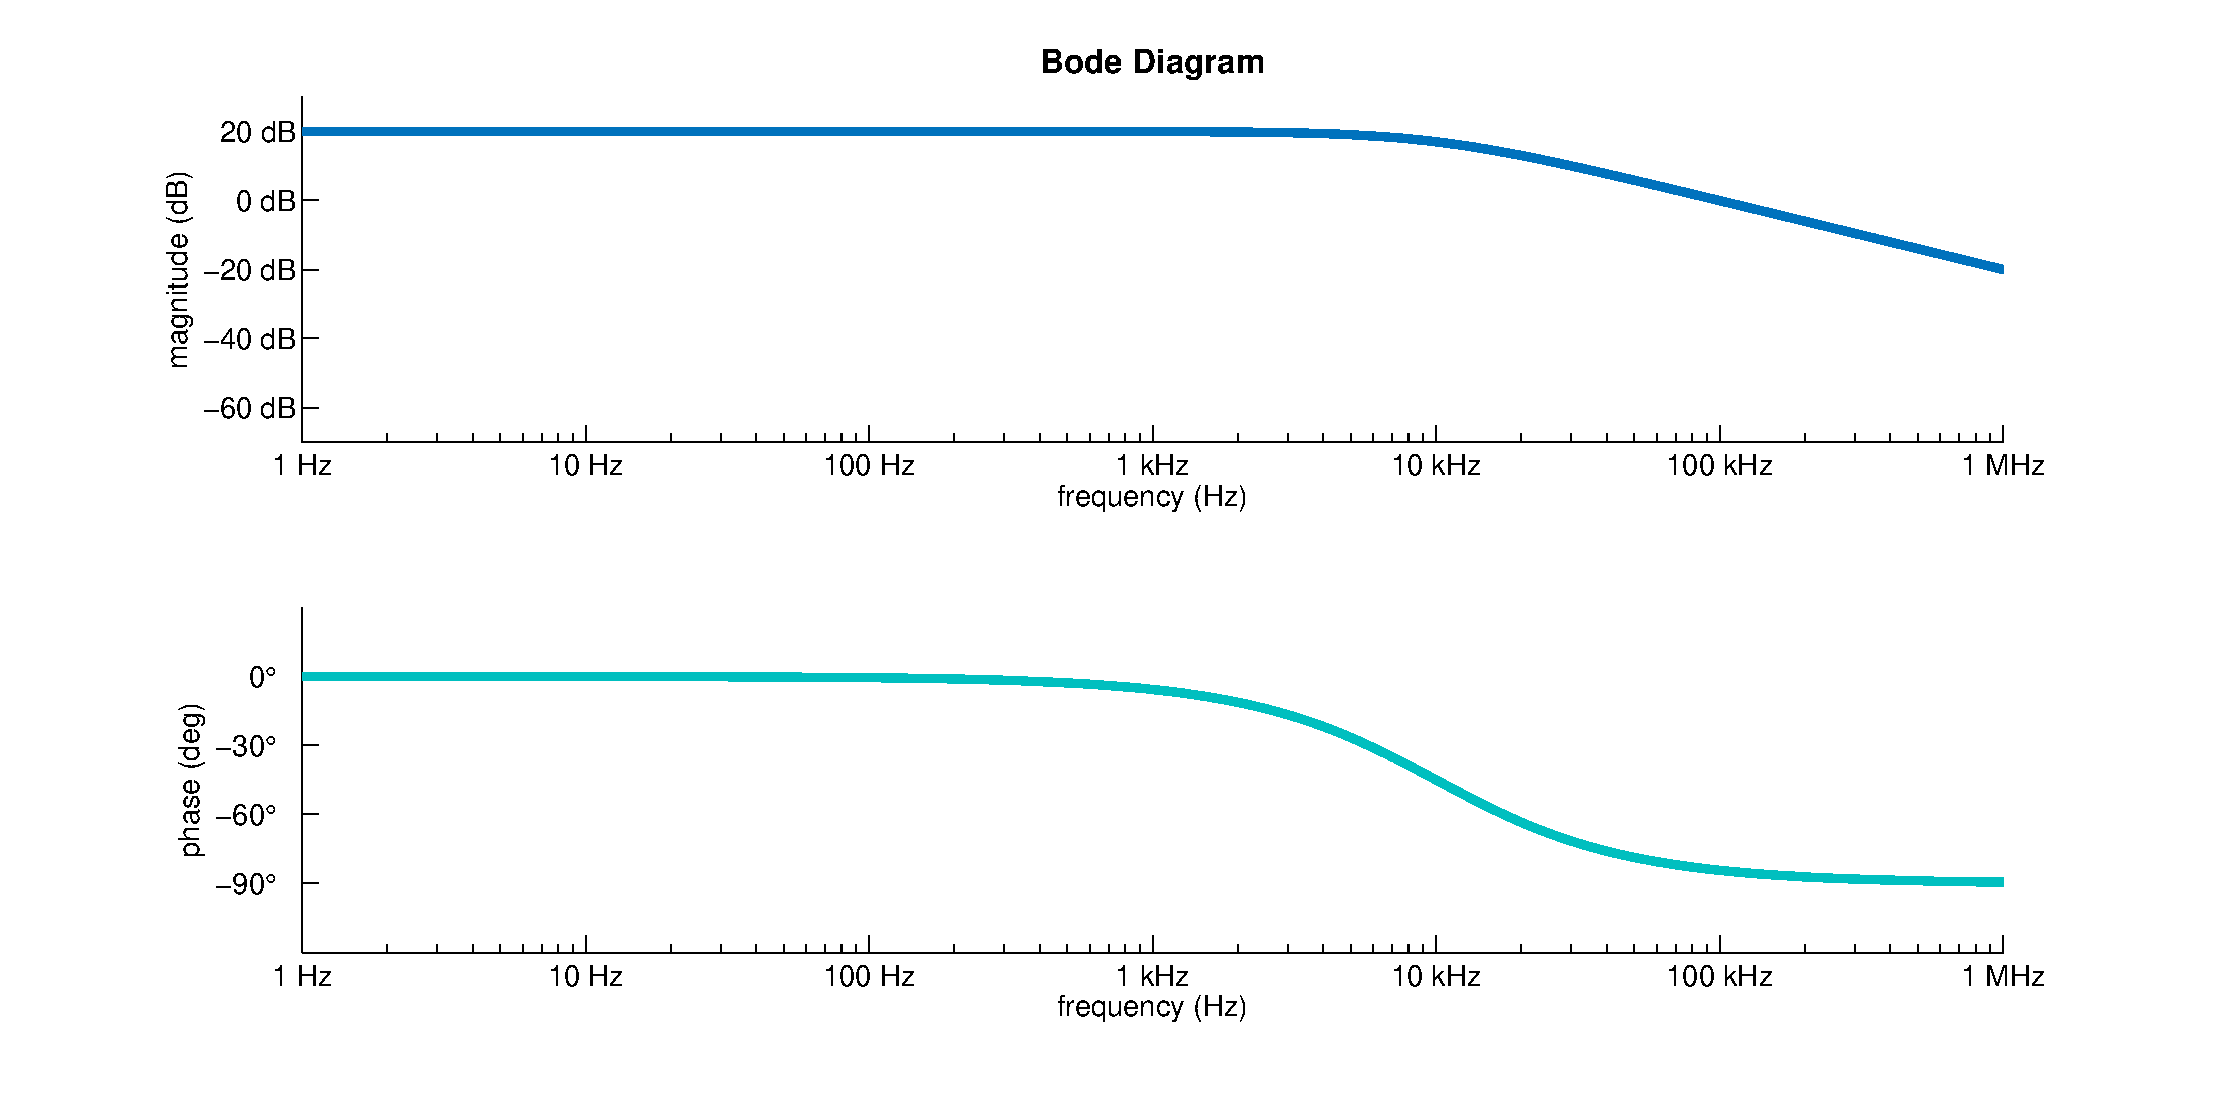
\includegraphics[width=\textwidth]{img/bodeDiagramOrdre1.eps}
%\caption{\label{fig:bode_ordre_1} Diagramme de Bode du premier ordre}
%\end{figure}
\newpage
\section{Non-idéalité des amplificateurs opérationnels}
Un amplificateur opérationnels est vu comme une source de tension commandée en tension
\begin{figure} [!h]
\centering
\input{circuit/op-amp.cir}
\caption{\label{schema_op_amp} Schéma d'un ampli op}
\end{figure} 
\\La fonction de transfert d'un ampli op est donnée par
\begin{equation}
V_\text{out} = g_fv_\varepsilon
\end{equation}
\subsection{Saturation}
La sortie d'un ampi-op est limitée par la tension d'alimentation $V_{CC}$ et $-V_{EE}$ : 
$$-V_{EE} < V_\text{Low} < V_\text{out} < V_\text{High} < V_{CC} $$

La courbe de transfert d'un ampli op est données par la figure \ref{fig:saturation}.
\begin{figure} [!h]
\centering
\input{img/saturation.figure}
\caption{\label{fig:saturation}Fonction de transfert d'un ampli op}
\end{figure}

\subsection{Impédances internes}
L'ampli op n'as pas une impédance infinie à l'entrée et nulle à la sortie. Si l'ampli op fonctionne en mode normal, il n'y a pas d'effet visible mais en mode saturé, cela a des effets sur le reste du circuit.
Le nouveau schéma de l'ampli op est donné à la figure \ref{fig:internal_impedance_op-amp}.
\begin{figure}[!h]
	\centering
	\input{circuit/op-amp-internal-resistors.cir}
	\caption{\label{fig:internal_impedance_op-amp}Impédance interne d'un ampli-op}
\end{figure}
\subsection{Limite du courant de sortie}
Dans le cas idéal, l'ampli-op est une source de tension parfaite avec une puissance infinie. Dans la réalité, le courant de sortie est limité à $I_\text{max}$. Tant que l'ampli-op, ne sature pas et que le courant de sortie reste inférieur à $I_\text{max}$, le cas idéal est une bonne approximation. Par contre, dans le cas où l'ampli-op sature, cela créer des non-linéarité. C'est à cause de la limite du courant de sortie, que la résistance de charge ne peut pas être trop faible.
\subsection{Réjection du mode commun}
La tension d'entrée de l'ampli op est : $V_\text{+}$ et $V_\text{-}$
On défini maintenant la tension différentielle : $V_\text{diff} = V_\text{+} - V_\text{-}$ et la tension de mode commun : $V_\text{comm} = \dfrac{V_+ + V_-}{2}$

À la sortie de l'ampli op , nous avons pour une légère différence entre $V_+$ et $V_-$ et un gain $A_\text{vd}$ 
\begin{equation}
V_\text{out} = A_\text{vd} \left(1+\frac{\varepsilon}{2}\right)V_+ - A_\text{vd} \left(1-\frac{\varepsilon}{2}\right)<V_- =A_\text{vd}(V_\text{diff}+\varepsilon V_\text{comm})
\end{equation}

\chapter{Puissance}
\section{Puissance instantanée, moyenne et valeur efficace}
\subsection{Puissance instantanée}
La puissance instantanée est le travail effectué par une charge $q$ par unité de temps. Le travail de cette charge $q$ est vu comme le déplacement d'une point $A$ à un point $B$ de la charge. On note ce travail comme $dW = dq \left(V_A-V_B\right)$. Avec l'expression du travail, la puissance s'exprime 
\begin{equation}
p=\dfrac{dW}{dt}=\dfrac{dq}{dt}\left(V_A-V_B\right)=i v
\end{equation}
La puissance peut être dépendante du temps : $p(t) = v(t) i(t)$\newline
Le dipôle absorbe de la puissance ($p>0$) si le courant et la tension sont dans le même sens ($i>0$ et $v>0$ ou $i<0$ et $v<0$). 
Dans le cas contraire, le dipôle fourni de la puissance.
\subsection{Puissance moyenne}
Dans le cas d'un courant périodique de période $T$, passant dans une résistance $R$, la puissance instantanée vaut $p(t)=i^2(t)R$. La puissance moyenne est définie comme 
\begin{equation}
P_\text{moy} = \frac{1}{T} \int_{t_0}^{t_0+T}{p(t)dT}
\end{equation}
Dans le cas d'un courant imposé à travers une résistance, cela nous donne 
$$ \frac{1}{T}\int_{t_0}^{t_0+T}{Ri^2(t)dT}$$
Dans le cas d'un courant sinusoïdale passant dans une résistance, nous avons comme puissance moyenne : 
$$P_\text{moy}=\frac{RI_\text{Max}^2}{2}=R\left(\frac{I_\text{Max}}{\sqrt{2}}\right)^2$$
\subsection{Valeur efficace}
\begin{itemize}
\item Courant : c'est le courant continu tel que la puissance dissipée dans la résistance ($RI_\text{eff}^2$) est égal à la puissance moyenne.
\begin{equation}
I_\text{eff}=\sqrt{\frac{P_\text{moy}}{R}}
\end{equation}
\item Tension : c'est la tension continue tel que la puissance dissipée dans la résistance ($V_\text{eff}^2/R$) est égale à la puissance moyenne.
\begin{equation}
V_\text{eff}=\sqrt{P_\text{moy} R}
\end{equation}
Pour un courant sinusoïdale, nous avons comme valeur efficace de la tension et du courant
$$ I_\text{eff}=\frac{I_\text{max}}{\sqrt{2}} \text{ et }  V_\text{eff}=\frac{V_\text{max}}{\sqrt{2}} $$
\end{itemize}
\subsection{Impédance quelconque}
Dans le cas d'un courant et d'une tension sinusoïdale dans une impédance quelconque, nous avons comme expression de la tension et du courant \newline
$v(t) = V_\text{max} \cos (\omega t + \psi_v)$\newline
$i(t) = I_\text{max} \cos (\omega t + \psi_i)$

La puissance instantanée s'écrit : 
$$p(t) = V_\text{max}I_\text{max} \cos (\omega t + \psi_v) \cos (\omega t + \psi_i) = \frac{1}{2}V_\text{max}I_\text{max} \left[\cos (\psi_v-\psi_i) + \cos(2\omega t + \psi_v + \psi_i)\right]$$
La puissance moyenne vaut
$$P_\text{moy}=\frac{1}{2}V_\text{max}I_\text{max} \cos (\psi_v-\psi_i) = V_\text{eff}I_\text{eff} \cos (\psi_v-\psi_i)$$
\section{Puissance active, réactive et apparente}
La puissance active \unit{P}{[\watt]} est définie comme la valeur moyenne de la puissance et traduit un échange unidirectionnel d'énergie entre la source et la charge.
\begin{equation}
P=V_\text{eff}I_\text{eff}\cos(\varphi)
\end{equation}
La puissance apparente \unit{S}{[Volt Ampère]} est définie comme l'amplitude de la composante fluctuante.
\begin{equation}
S=V_\text{eff}I_\text{eff}
\end{equation}
La puissance réactive \unit{Q}{[Volt Ampère Réactif]} traduit un échange bidirectionnel d'énergie entre la source et la charge. !!! Ce n'est valable qu'en régime sinusoïdale !!!
\begin{equation}
Q=V_\text{eff}I_\text{eff}\sin(\varphi)
\end{equation}

\chapter{Circuit magnétique couplé}
\section{Inductance}
Soit une bobine de $N$ spire et traversée par un courant $i$. Alors un champ magnétique ($\vec{B}$) est généré. Au champ magnétique correspond un flux $\phi$  sur une spire. Il est donné par la relation
\begin{equation}
\phi=\int_\text{S}{\vec{B}\vec{dS}}
\end{equation}
Le flux total sur tout le bobinage est donné par 
\begin{equation}
\Phi=N\phi
\end{equation}
\end{document}
